\chapter{State of the Art}
\label{chap:state-of-the-art}

\lettrine[lines=3, findent=3pt, nindent=0pt]{T}{his} chapter rounds out the theoretical background and technologies used in the project and discussed in the following: beginning with how network traffic is made ad how to characterize malicious activities, it will then be discussed Software Defined Networking as an industry standard and then Machine Learning will be introduced, with particular emphasis on Intrusion Detection applications of Deep Learning. The reader should here be provided with sufficient knowledge to understand chapters \ref{chap:methodology}, \ref{chap:results} and \ref{chap:conclusions}.

%----------------------------------------------------
% NETWORK TRAFFIC
%----------------------------------------------------

\section{Network Traffic}
\label{sec:network-traffic}

\textit{Network Traffic} is the amount of data that passes through a network at a given time, and it represents the starting point to the project. \\ Network architecture was thought to be modular and explicit, to ensure that modifications made to a single component were transparent to the rest of the system. This modularization is represented by \textit{network protocols} being separated into different layers: each layer has a precise task. In 1960s the \textit{U.S. Department of Defense} designed the \textit{TCP/IP} model, which is now the \textit{de facto} standard for protocols stack. Network security should be addressed at each TCP/IP network layer for different vulnerabilities and attack types \cite{Zaman2009}.

\begin{figure}[h!]
    \centering
    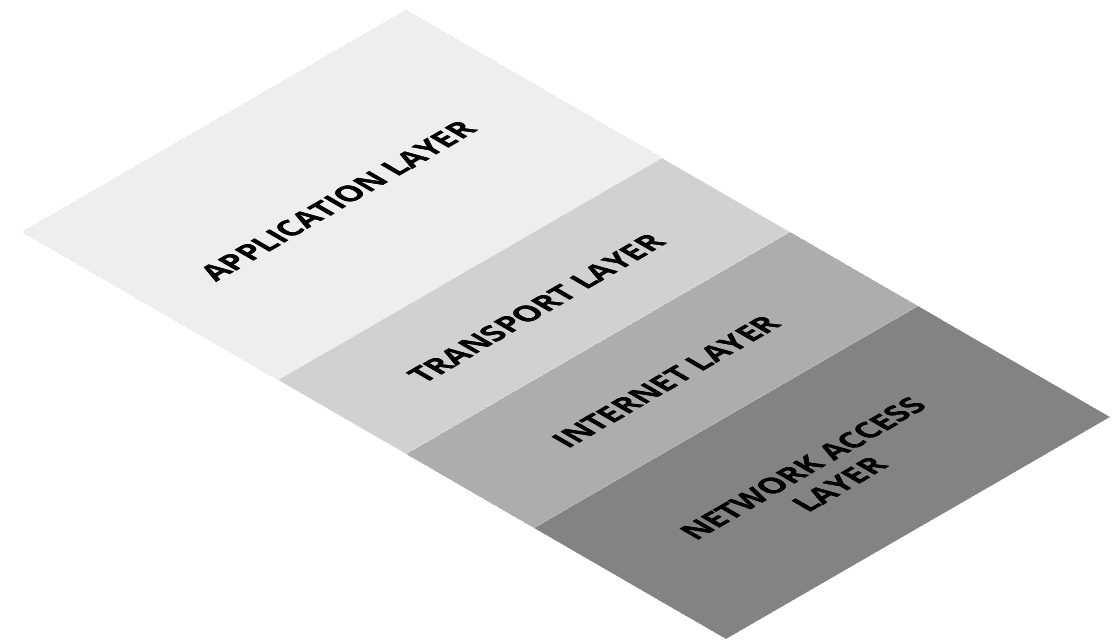
\includegraphics[scale=0.23]{figures/TCP_IP Stack.png}
    \caption{Internet protocol suite: TCP/IP Stack}
    \label{fig:TCP/IP-stack}
\end{figure}

\textit{TCP/IP} stack is composed of 4 layers, representing from the physical connection (\textit{Network Access Layer}) to the user interface (\textit{Application Layer}). \\ The most relevant layer for this project is the third one: \textit{Transport Layer}, also called \textit{Host to Host Layer} is responsible for end-to-end communication and error-free delivery of data. It shields the upper-layer applications from the complexities of data. The main protocols used in this layer are:

\begin{itemize}
    \item[\faCaretRight] \textit{Transmission Control Protocol} (TCP): provides reliable and error-free communication between end systems. It also has acknowledgement features and a flow control system. This protocol has a lot of overhead due to its features;
    \item[\faCaretRight] \textit{User Datagram Protocol} (UDP): unlikely TCP, this protocol doesn't ensure a reliable connection between points, but it is very cost effective and lightweight.
\end{itemize}
Network packets are encapsulated in either a \textit{TCP segment} or a \textit{UDP datagram}. Another relevant protocol that will be used is \textit{Internet Control Message Protocol} (ICMP), belonging to the second layer (\textit{Internet Layer}): it s responsible for providing hosts with information about network problems. Because of this particular design of network architecture, in which one layer acts as an intermediate between the layer above, and the one below, when trying to characterize the traffic, looking only at these latter protocols can be sufficient \cite{Iglesias2015}.

%----------------------------------------------------
% MALICIOUS TRAFFIC
%----------------------------------------------------

\subsection{Malicious Network Traffic}
\label{subsec:malicious-traffic}

An \textit{intrusion} can be defined as an attempt to access information about computer systems ot to damage system operation in an illegal or unauthorized manner \cite{Liu2019}, hence it will be considered \textit{malicious traffic} the entirety of network traffic generated by such operations. \\
The classes of malicious traffic analyzed in this work are te following:

\begin{itemize}
    \item[\faCaretRight] \textit{Bruteforce}: this kind of attack is one of the most popular and it can be used to guess passwords or URLs (in order to discover hidden contents in web applications). It can be defined as an hint and try attack \cite{icissp18};
    \item[\faCaretRight] \textit{Botnet}: a botnet is a number of Internet connected devices, used to perform various tasks, from stealing data, to spam, or to practice \textit{Distributed Denial of Service} (DDoS) attacks \cite{icissp18};
    \item[\faCaretRight] \textit{Cross-site-scripting} (XSS): this kind of vulnerability can typically be found in web applications. An XSS attack consist of injecting client-side scripts into web pages, that can be viewed by other users;
    \item[\faCaretRight] \textit{Denial of Service} (DoS): this type of attack foresees the overloading of a network infrastructure, denying or preventing legitimate users to access resources on the system or the network \cite{Sharafaldin2019};
    \item[\faCaretRight] \textit{Distributed Denial of Service} (DDoS): POINT OUT COMMON TOOLS (EG SLOWLORIS)
    \item[\faCaretRight] \textit{Heartbleed}: this particular attack exploits a bug in the OpenSSL cryptography library (widely used implementation of the \textit{Transport Layer Security} protocol) and it can bla bla discovered in 2014 bla bla \cite{icissp18}, \cite{Carvalho2014} and \cite{Stallings2014};
    \item[\faCaretRight] \textit{Port Scanning}: this occurs when an attacker sends probe packets to gather intelligence information about the infrastructure, based on the responses received;
    \item[\faCaretRight] \textit{SQL-Injection}: malicious database queries can be used to extract bulk data from the latter; this can occur, fro example, through badly projected forms on web pages.
\end{itemize}
The dataset\footnote{See section \ref{subsec:datasets-for-evaluation}} used bla bla

%----------------------------------------------------
% TRAFFIC CHARACTERIZATION
%----------------------------------------------------

\subsection{Traffic Characterization}
\label{subsec:traffic-characterization}

See paper \cite{Iglesias2015} and  \cite{Velan2016} \\ Openflow

\lipsum

%----------------------------------------------------
% SOFTWARE DEFINED NETWORKING
%----------------------------------------------------

\section{Software Defined Networking}
\label{sec:sdn}

\lipsum

%----------------------------------------------------
% INTRUSION DETECTION SYSTEMS
%----------------------------------------------------

\section{Intrusion Detection Systems}
\label{sec:intrusion-detection-system}

\lipsum[1-5]

    \begin{figure}[h!]
        \centering
        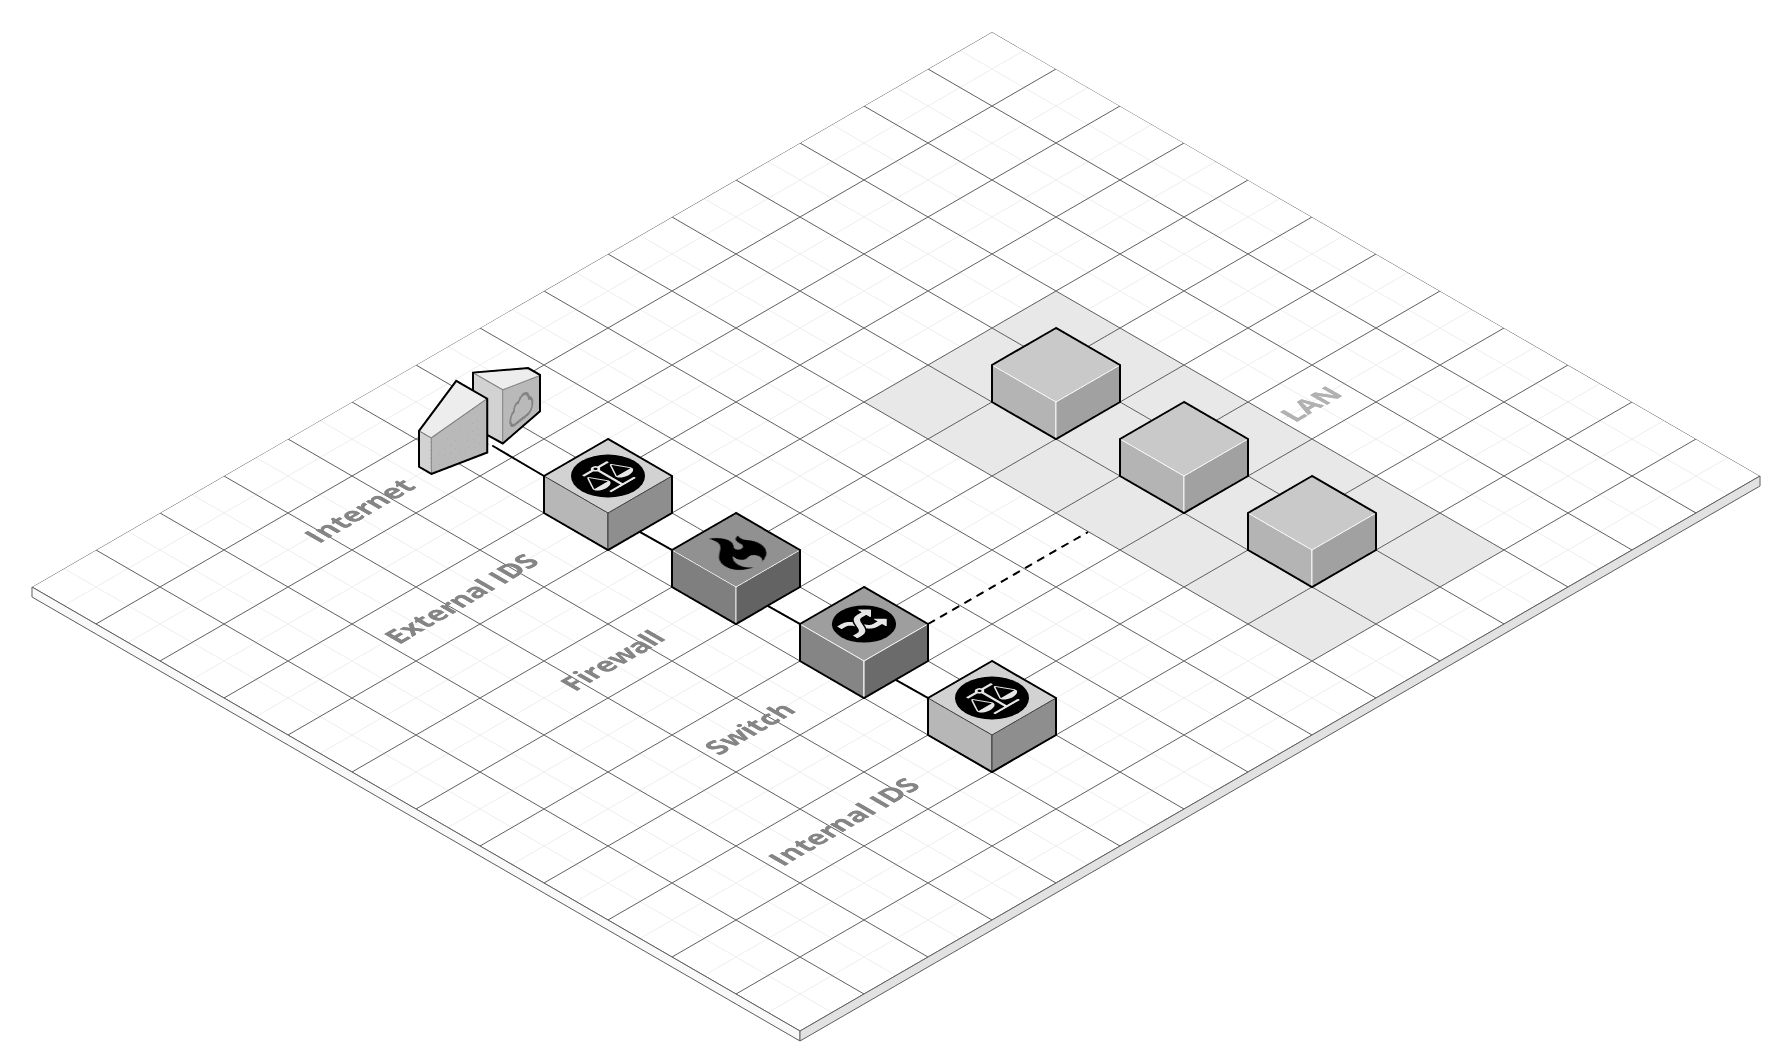
\includegraphics[scale=0.23]{figures/Intrusion Detection System Model.png}
        \caption{Intrusion Detection System Model}
        \label{fig:IDS-model}
    \end{figure}

%----------------------------------------------------
% TAXONOMY OF INTRUSION DETECTION SYSTEMS
%----------------------------------------------------

\subsection{Taxonomy of Intrusion Detection Systems}

See paper \cite{Liu2019}

%----------------------------------------------------
% DATASETS FOR INTRUSION DETECTION SYSTEMS
%----------------------------------------------------

\subsection{Datasets for Intrusion Detection Evaluation}
\label{subsec:datasets-for-evaluation}

See paper \cite{icissp18}, \cite{Khraisat2019} and \cite{Leevy2020} \\

\lipsum[1-6]

%----------------------------------------------------
% MACHINE LEARNING
%----------------------------------------------------

\section{Machine Learning}
\label{sec:machine-learning}

See paper \cite{Khraisat2019} and \cite{Hodo2017} \\

\lipsum \\
Discussed in \ref{sec:machine-learning}

%----------------------------------------------------
% MACHINE LEARNING ALGORITHMS
%----------------------------------------------------

\subsection{Machine Learning Algorithms}
\label{subsec:ml-algorithms}

\lipsum

%----------------------------------------------------
% DEEP LEARNING
%----------------------------------------------------

\subsection{Deep Learning}
\label{subsec:deep-learning}

\lipsum

%----------------------------------------------------
% MACHINE LEARNING LIBRARIES
%----------------------------------------------------

\subsection{Machine Learning Libraries}
\label{subsec:ml-libraries}

\lipsum